\documentclass{article}

\usepackage[english]{babel}
\usepackage[utf8]{inputenc}
\usepackage{fancyhdr}
\usepackage{amsmath}
\usepackage{amssymb}
\usepackage{setspace} 
\usepackage{graphicx}
\usepackage{float}
\usepackage{tabularx}


\pagestyle{fancy}
\fancyhf{}
\lhead{CIV102: Formula sheet}
\rhead{Youssef El Mays}
\doublespacing



\newcommand{\SubItem}[1]{
    {\setlength\itemindent{15pt} \item[-] #1}
}

\newcolumntype{L}{>{\centering\arraybackslash}m{3cm}}


\begin{document}
    \title{CIV102: Formula Sheet}

    \section{Stress, Strain}
        \begin{flalign} 
            &\sigma = \frac{F}{A} &\\
            &\epsilon = \frac{\Delta l}{L} &\\
            &\sigma = E\epsilon  &\\
            &\frac{F}{A} = \frac{E \cdot \Delta l}{L}, F = \frac{AE}{L} \cdot \Delta l = k \Delta l  \\
            &k = \frac{AE}{L}  &\\
            &W = \frac{1}{2}k\Delta x^2 
            = \frac{1}{2} F\Delta x 
            = \frac{1}{2} \sigma A \epsilon L 
            = \frac{\sigma^2 V_0}{2E} 
            = \frac{\sigma \epsilon V_0}{2}&\\ 
            &U = \int \sigma d\epsilon &\\
            &W = U \cdot V_0 \rightarrow U = \frac{W}{V_0} &\\
            &\epsilon_{th} = \alpha \Delta T& \\
            &F_{failure} = A\sigma_y& \\
            &F_{allowable} = \frac{A\sigma_y}{FOS} \geq F_{demand} &\\
            &A \geq \frac{FOS \cdot F_{demand}}{\sigma_y}&
        \end{flalign}

    \section{Equilibrium}  
        \begin{flalign}
            &\Sigma F = 0,\;
            \Sigma M = 0,\;if\;a = 0, &\\
            &\;where\;F = ma,\;and\;M = Fd&
        \end{flalign}
    
    \section{Bridges}
        \begin{flalign}
           & T_{supY}=\frac{WL}{2}& \\
           & T_{supX}=\frac{WL^{2}}{8h}& \\
           & T_{supMax}=\sqrt{(\frac{WL}{2})^{2} + (\frac{WL^{2}}{8h})^2},& 
        \end{flalign}
        Given loads placed equidistantly over the span

    \section{Rotation}
        \subsection{Motion}
        \begin{flalign}
           & I_{m} = my^{2},\;for\;a\;single\;point\;mass\\
           & I_{m} = \int_{M} y^2 dm = \rho \int_A y^2 dA &\\
           & I = \int_A y^2 dA&\\
           & I = \frac{bh^3}{12}, \;for\;a\;rectangle\;(comes \;from\;integrating)& \\
           & F=ma=my&\\
           & M=F_{x}y=my^{2} \cdot \alpha = I_{m}\alpha &\\
           & \omega = \frac{d^{2}\theta}{dt^{2}}& \\
           & \theta = \omega_{i}t + \frac{1}{2}\alpha t^{2}&\\   
           & a = \alpha y& \\
           & M = Fy = m\alpha y^2 = I_m \alpha&
        \end{flalign}
        \subsection{Bending}
        \begin{figure}[H]
            \centering
            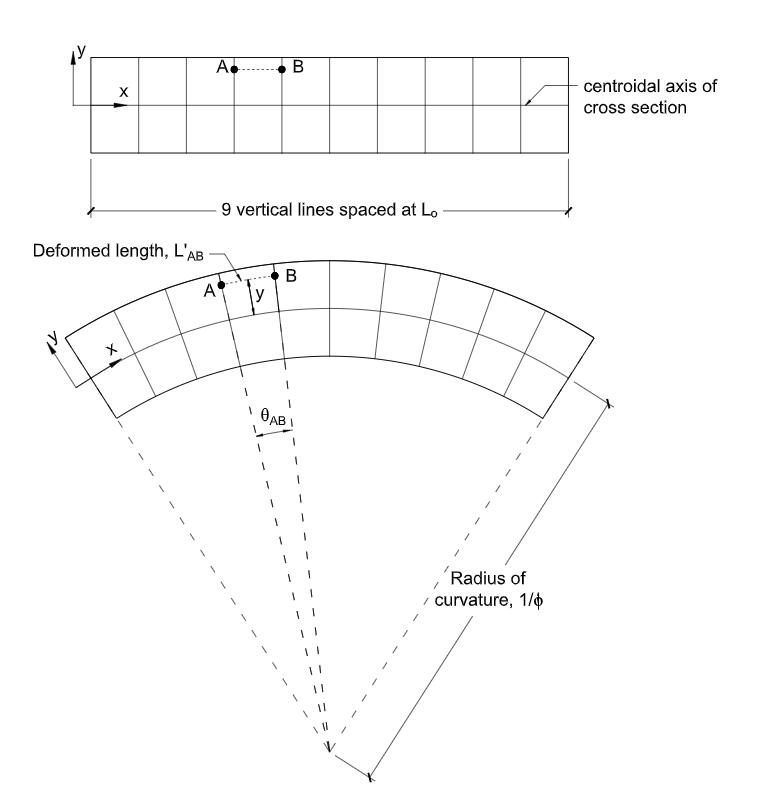
\includegraphics[width=6cm]{Bending.png}
        \end{figure}
        \begin{flalign}
           & \phi = \frac{d\theta}{dx} &\\
           & L^\prime_{AB} = \phi L_0 \cdot (y +\frac{1}{\phi}) = \phi y L_0 + L_0 &\\
           & \epsilon(y) = \frac{\Delta l}{L_0} = \frac{L^\prime_{AB} - L_0}{L_0} = \phi y,\;\epsilon\; at\; the \; centroidal\; axis\; is\;0&\\
           & \sigma = E\epsilon \rightarrow \sigma(y) = E\phi y &\\
           & \sigma = F/A \rightarrow \Delta F = \sigma(y)\Delta A &\\
           & M =Fd \rightarrow \Delta M = \Delta Fy = \phi E y^2 \Delta A &\\
           & M = \int_A \phi E y^2 dA = \phi E I&
        \end{flalign}

    
    \section{Harmonic Motion}
        \begin{flalign}
            &Pendulum:\;T = 2\pi \sqrt{\frac{l}{g}} &\\
            &Mass\;Spring:\;2\pi \sqrt{\frac{m}{k}} &\\
            &f = \frac{1}{T} &\\
            &F = -kx &\\
            &\omega = \frac{2\pi}{T}& \\
            &a = -\omega^2 x &\\
            &x(t) =A \cdot \sin(\omega t + \phi) &\\
            &v = \omega A \cdot \cos(\omega t + \phi)& \\
            &v = \pm \omega \sqrt{x_0^2 - x^2}& \\
            &\frac{d^2x(t)}{dt^2} = -A\omega^2 \sin(\omega_n t + \phi)& \\
            &E_k = \frac{1}{2}m\omega^2 (x_0^2 - x^2) &\\
            &E_t = \frac{1}{2}m\omega^2 x^2& \\
            &\frac{1}{2}mv^2 = \frac{1}{2}kx^2 \rightarrow v = \sqrt{x\frac{k}{m}}&
        \end{flalign}

        \textbf{Gravity}
        \begin{flalign}
            &m\frac{d^2x(t)}{dt^2} + kx(t)=mg& \\
            &x(t) = A \sin(\omega_nt + \phi) + \Delta_0 &\\
            &k = \frac{mg}{\Delta_0} &\\
            &f_n = \frac{1}{2\pi}\sqrt{\frac{mg}{\Delta_0}\cdot\frac{1}{m}} =\frac{1}{2\pi}\sqrt{\frac{g}{\Delta_0}}&
        \end{flalign}

    \section{Staticaly Determined Structures}
        \begin{table}[H]
            \centering
            \begin{tabularx}{\textwidth}{| X | L | L | c |}
                \hline
                \textbf{Name} & 
                \textbf{Permited Degrees of Freedom} & 
                \textbf{Restrained Degrees of Freedom} &
                \textbf{Reactions} \\
                \hline
                Roller & 
                $\Delta(x \oplus y),\;\theta$ &
                $\Delta y = 0$ &
                $F_y$ \\
                \hline
                Pin &
                $\theta$ &
                $\Delta x = \Delta y = 0$ &
                $F_x,\;F_y$ \\
                \hline 
                Fixed End &
                N/A &
                $\Delta x = \Delta y = \Delta \theta = 0$ &
                $F_x,\;F_y,\;M_{xy}$ \\
                \hline
            \end{tabularx}
        \end{table}

    \section{Truss Brigde}
        \begin{figure}[H]
            \centering
            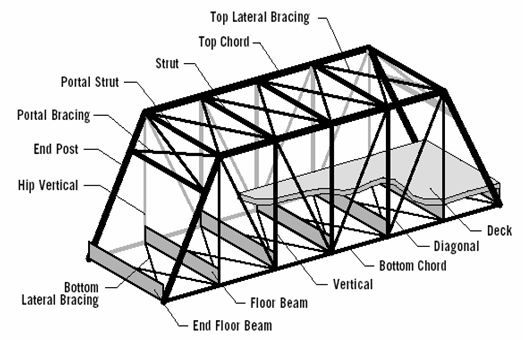
\includegraphics[width=8cm]{TrussBridge.jpeg}
        \end{figure}
        \begin{enumerate}
            \item Select Geometry
            \item Determine Loads
                \SubItem{Gravity}
                \SubItem{Wind}
            \item Analyze forces in members
            \item Design components
            \item Determine stiffeness
            \item Check dynamic forces 
            \item Iterate
        \end{enumerate}
        \begin{flalign}
            &P_{central\;joint}= W \cdot \frac{s\cdot W_D}{2} &\\
           & P_{end\;joint}= W \cdot \frac{s\cdot W_D}{4} &\\
           & \textbf{Deflection:}\\
            &W_{ext} = \sum^m_{i=1}{\int F_i d\Delta_i}\;m\;Forces& \\
            &W_{int} = \sum^n_{i=1}{\int P_i d\Delta_i}\; n \;members& \\
            &W_{ext} = W_{int} &\\
            &F^\star = virtual\; force &\\
           & \Delta_l = \frac{PL}{AE} &\\
            &F^\star \Delta = \sum{P^\star \Delta_l} = \sum{P^\star  \frac{PL}{AE}} &\\
            & \text{Loads from people/crowd} = 5Mpa& 
        \end{flalign}
    
    \section{Buckling}
        \begin{flalign}
           & \phi = \frac{d\theta}{dx} &\\
           & P \cdot y = P \cdot \Delta_{lat} = M&\\
           & M = EI\phi &\\
           & y(x) = A \sin(\omega x + B) &\\
            &\frac{dy}{dx} = A\omega \cos(\omega x +B) &\\
           & \frac{d^2y}{dx^2} = -A\omega^2 \sin(\omega x +B)& \\
            &n\pi =L\cdot \sqrt{\frac{P}{EI}},\;n\;\epsilon \;\mathbb{N}&\\
            &P = \frac{n^2\pi^2 E I}{L^2}& \\
            &P_{crit} = \frac{\pi^2 EI}{L^2} = P_E &\\
            &r = \sqrt{\frac{I}{A}},\;r=\;radius\;of\;gyration&\\
            &\sigma_E = \frac{P_E }{A} = \frac{\pi^2 EI}{AL^2} = \frac{\pi^2 E}{(L/r)^2},\;L/r=\;slenderness\;ratio & \\
            &L/r < 200
        \end{flalign}
    \section{Combined loads}
        \begin{flalign} 
           & \sigma_t = \sigma_N + \sigma_M = \frac{N}{A} + \frac{My}{I} & \\
           & \text{Moment at base of eccentric structure: } M = eP
        \end{flalign}

    \section{Compression Member}
    \begin{flalign}
        &failure\;envelope = \min\{\sigma_y, \sigma_E\} &\\
        &\sigma_{allowable} = \min\{\frac{1}{FOS_{crush}}\cdot\sigma_y, \frac{1}{FOS_{buckling}}\cdot\sigma_E\} &\\
        &Yield:\;F_{allowable}=\frac{1}{FOS_{crush}}A\sigma_Y \geq F_{demand}& \\
        &A \geq FOS_{crush} \cdot \frac{F_{demand}}{\sigma_Y}&\\
        &Buckling:\;F_{allowable}=\frac{1}{FOS_{buckling}}A\sigma_E \geq F_{demand} &\\
        &I \geq FOS_{buckling} \cdot \frac{F_{demand} L^2}{\pi^2 E}&
    \end{flalign}

    \section{Wind}
    \begin{flalign}
       & W_{wind} = \frac{F_{wind}}{A} = \frac{1}{2}\rho v^2 C_D &\\
        &race\;car:\;C_D=0.2&\\
        &sphere:\;C_D=0.75 &\\
        &boxy\;object:\;C_D=1.5& \\
        &\rho_{air} = 1.2kg/m^3& \\
        &C_D = 1.5 &\\
        &V \geq 170km/h \approx 47.2m/s &\\
        &W_{wind\;ave} = 2.0kPa&\\
        &A_{tributary\;bottom} = \frac{h \cdot s}{2},\; due \; to\; handrail &\\
        &A_{tributary\;top} = \Sigma sh&
    \end{flalign}

    \section{Free vibrations in truss}
    \begin{flalign}
        &f_n = \frac{15.76}{\sqrt{\Delta_0}}\; for\; single\; load& \\
        &f_n = \frac{17.76}{\sqrt{\Delta_0}}\; for\; distributed\; load&\\
        &\textbf{Damping}: \text{Tendency of a system to lose energy as it vibrates} &\\
        &\beta = \text{Damping ratio} \\
        &\frac{m d^2x}{dt^2} + 2\beta\sqrt{mk}\frac{dx}{dt} + kx = mg &\\
        &x(t) = Ae^{-\beta \omega_n t} sin(\omega_n t \sqrt{1 - \beta^2} + \phi) + \Delta_0&
    \end{flalign}

    \section{Forced vibrations}
    \begin{flalign}
        &F(t) = F_0sin(\omega t)+mg &\\
        &\frac{m d^2x}{dt^2} + 2\beta\sqrt{mk}\frac{dx}{dt} + kx = F_0sin(\omega t) mg &\\
        &x(t) = DAF \cdot \frac{F_0}{k}\sin(\omega t + \phi) + \Delta_0,\;\text{At steady state} &\\
        &\textbf{Dynamic Amplification Factor}:\; DAF = \frac{1}{\sqrt{(1-(\frac{f}{f_n})^2)^2+(2\frac{\beta f}{f_n})^2}}&\\
        &\Delta_{max} = \frac{F_{max}}{k}& \\
        &F_{max} = DAF \cdot F_0 + mg &
    \end{flalign}

    \section{Shear forces}
    \begin{flalign}
        &w(x) = \frac{d}{dx}v(x)& \\
        &\Delta V_{12} = \int_{x1}^{x2}w(x) \,dx& \\
        &v(x) = \frac{d}{dx}M(x)& \\
        &\Delta M_{12} = M_2 - M_1 = \int_{x1}^{x2}v(x)\,dx & 
    \end{flalign}

    \section{Shear Stress}
    \begin{flalign}
        & \tau = \; \text{Shear Stress}& \\
        & \Delta C = \tau \cdot b \Delta x = \int \sigma \,dA &\\
        & \tau \cdot b \Delta x = \int_{y_0}^{y_{top}} \frac{\Delta M y}{I}\,dA =\frac{\Delta M}{I} \cdot \int_{y_0}^{y_{top}} y\,dA & \\
        & \tau = \frac{\Delta M}{\Delta x} \cdot \frac{1}{Ib} \cdot \int_{y_0}^{y_{top}} y\,dA =  \frac{\Delta M}{\Delta x} \cdot \frac{Q}{Ib} &\\
        & V = \frac{dM}{dx} & \\
        & \tau = \frac{VQ}{Ib} & \\
        & Q =\;\text{First Moment of Area taken about the centroid} &\\
        & Q = \int_{y_0}^{y_{top}} y\,dA = \int_{y_{bot}}^{y_{0}} y\,dA \eqsim \sum_{i=0}^n A_i d_i & \\
        & A_i = \text{areas of cross section from $y_0$ to top/bottom of cross section} & \\
        & d_i = \text{distance from centroid of $A_i$ to centroidal axis of cross section} & \\
        & Q = \frac{1}{2}by(h - y) \; \text{for rectangle} & \\
        & Q(0) = Q(h) = 0 & \\
        & \frac{dQ}{dy}(\frac{h}{2}) = 0
    \end{flalign}

    \section{Flexural Stresses}
    \begin{flalign}
        &\Delta l =0\; \text{at centroidal axis}& \\
        &\phi = \frac{d\theta}{dx} = \frac{d}{dx}(\frac{dy}{dx}) = \frac{d^2y}{dx^2},\;\phi=\text{curvature}& \\
        &\epsilon(y) = \phi y &\\
        &I = \int y^2dA& \\
        & \sigma = E\epsilon&\\
        &\sigma(y) = E \phi y & \\
        & \Delta F_i = \sigma_i \Delta A_i = E \phi y \cdot \Delta A_i & \\
        & N = \sum_{i=0}^n \Delta F_i = 0 &\\
        & 0 = \sum_{i=0}^n E\phi y_i \Delta A_i &\\
        & \lim_{\Delta A \rightarrow 0} \sum_{i=0}^n E\phi y_i \Delta A_i = \int E \phi y\,dA&\\
        & \Delta M_i = \Delta F_i y_i &\\
        & M = \lim_{\Delta A \rightarrow 0} \sum_{i=0}^n \Delta F_i y_i = \lim_{\Delta A \rightarrow 0} \sum_{i=0}^n E \phi y^2_i \cdot \Delta A_i = E\phi \int y^2_i dA &\\
        &M = EI\phi = EI \frac{\sigma}{Ey} = EI (\frac{d^2y}{dx^2})& \\
        & \sigma  = \frac{My}{I},\;\textbf{Navier's equation},\;&\\
        &M = \text{bending Moment},\; I = \text{Second Moment of area}& \\
       & \sigma = \text{Flexural stress},\;y = \text{Vertical Distance from centroid} & \\
       & \Delta \theta_{12} = \theta_2 - \theta_1 = \int_{x_1}^{x_2} \phi\,dx \\
       & \delta_{DT} = \lim_{\Delta x \rightarrow\infty}\sum_{i = 1}^n \phi(x_i)(x_{DT} - x_i)\Delta x = \int\phi(x)(x_{DT} - x)dx 
    \end{flalign}

    \section{Poisson and Plate }
    \begin{flalign}
        & \epsilon_{x\,poission} = -\mu \frac{\sigma_y}{E} &\\
        & \epsilon_{y\,poission} = -\mu \frac{\sigma_x}{E} &\\    
        & \epsilon_x = \frac{\sigma_x}{E} - \mu \frac{\sigma_y}{E} &\\    
        & \epsilon_y = \frac{\sigma_y}{E} - \mu \frac{\sigma_x}{E} & \\
        & y = A\cdot \sin{(\frac{n\pi}{L}X)}, n \epsilon & \\
        & P_E = \frac{\pi^2EI}{L^2} & \\
        & I = \frac{bt^3}{12},\; A=bt &\\
        & P_E = \frac{\pi^2E}{L^2} \cdot  \frac{bt^3}{12} & \\
        & \sigma_E = \frac{P_E}{A} = \frac{\pi^2E}{12} \cdot \left(\frac{t}{L}\right)^2 & \\
        & z = a\sin{(\frac{m\pi x}{b}) \sin{(\frac{n\pi y}{L})}} &\\
        & \sigma_{crit} = \frac{k\pi^2E}{12(1-\mu^2)}\cdot\left(\frac{t}{b}\right)^2 & \\
        & \textbf{Support conditions} & \\
        & z = 0 &\\
        & \sigma_{crit} = \frac{4\pi^2 E}{12(1-\mu^2)} \cdot \left(\frac{t}{b}\right)^2 & \\
        & z \neq 0 \;\text{on one side} &\\
        & \sigma_{crit} = \frac{0.425\pi^2 E}{12(1-\mu^2)} \cdot \left(\frac{t}{b}\right)^2 & \\
        & z = 0 &\\
        & \text{Stress varies liearly from 0 to $\sigma_{crit}$} & \\
        & \sigma_{crit} = \frac{6\pi^2 E}{12(1-\mu^2)} \cdot \left(\frac{t}{b}\right)^2 & \\
        & \tau_{crit} = \frac{5\pi^2E}{12(1-\mu^2)} \cdot \left[\left(\frac{t}{h}\right)^2 + \left(\frac{t}{a}\right)^2\right]
    \end{flalign}

    \section{Reinforced Concrete}
    \begin{flalign}
        & f'_t  =0.33\sqrt{f^\prime_c} & \\
        & Ec = 4730\sqrt{f^\prime_c} &  \\
        & b = \text{width of section on compression side} & \\
        & A_s = \text{total area of longitudinal steel on tension side } & \\
        & d = \text{distance to $A_s$ from the compression side} & \\
        & kd = \text{depth of compression} & \\
        & jd = \text{flexural lever arm} & \\
        & \epsilon = \phi y & \\
        & C_c = \int fdA & \\
        & T_s = f_s \cdot As & \\
        & |T_s| = |C_c| &\\
        & M = jd \cdot C_c = jd \cdot T_s &\\
        & k = \sqrt{\left(n\rho\right)^2 + 2n\rho} - n\rho &\\
        & n = \frac{E_s}{E_c},\;\text{modular ratio} &\\
        & \rho  = \frac{As}{bd} & \\
        & j = 1 - \frac{1}{3}k & \\
        & f_s = \frac{M}{As\cdot jd} & \\
        & f_c = \frac{k}{1 - k} \cdot \frac{M}{jd \cdot As \cdot n} & \\
        & V_{ult} = V_c + V_s \leq V_{max} & \\
        & V_{safe} 0.5V_c + 0.6V_s \leq 0.5 V_{max} & \\
        & V_{max} 0.25f^\prime_cb_w \cdot jd & \\ 
        & \text{No Shear reinforcement: } V = \frac{230 \sqrt{f^\prime_c}}{1000 + 0.9d} \cdot b_wjd & \\
        & \text{Shear reinforcement: } &\\
        & V = \frac{Av f_y jd}{s} \cdot \cot{\left(35^\circ \right)}& \\
        & V_c = 0.18 \sqrt{f^\prime_c } b_wjd\;if\;\frac{AvF_y}{b_w s} \geq 0.06\sqrt{f^\prime_c}
    \end{flalign}
\end{document}
